\chapter{Applications and transport agent API}
\label{chap:applications}

Applications sit on top of transport agents in \ns.  There are two basic types
of applications:  traffic generators and simulated applications.  
Figure~\ref{fig:application} illustrates two examples of how applications
are composed and attached to transport agents.  Transport agents are described
in Part V (Transport).

\begin{figure}[tb] 
  \centerline{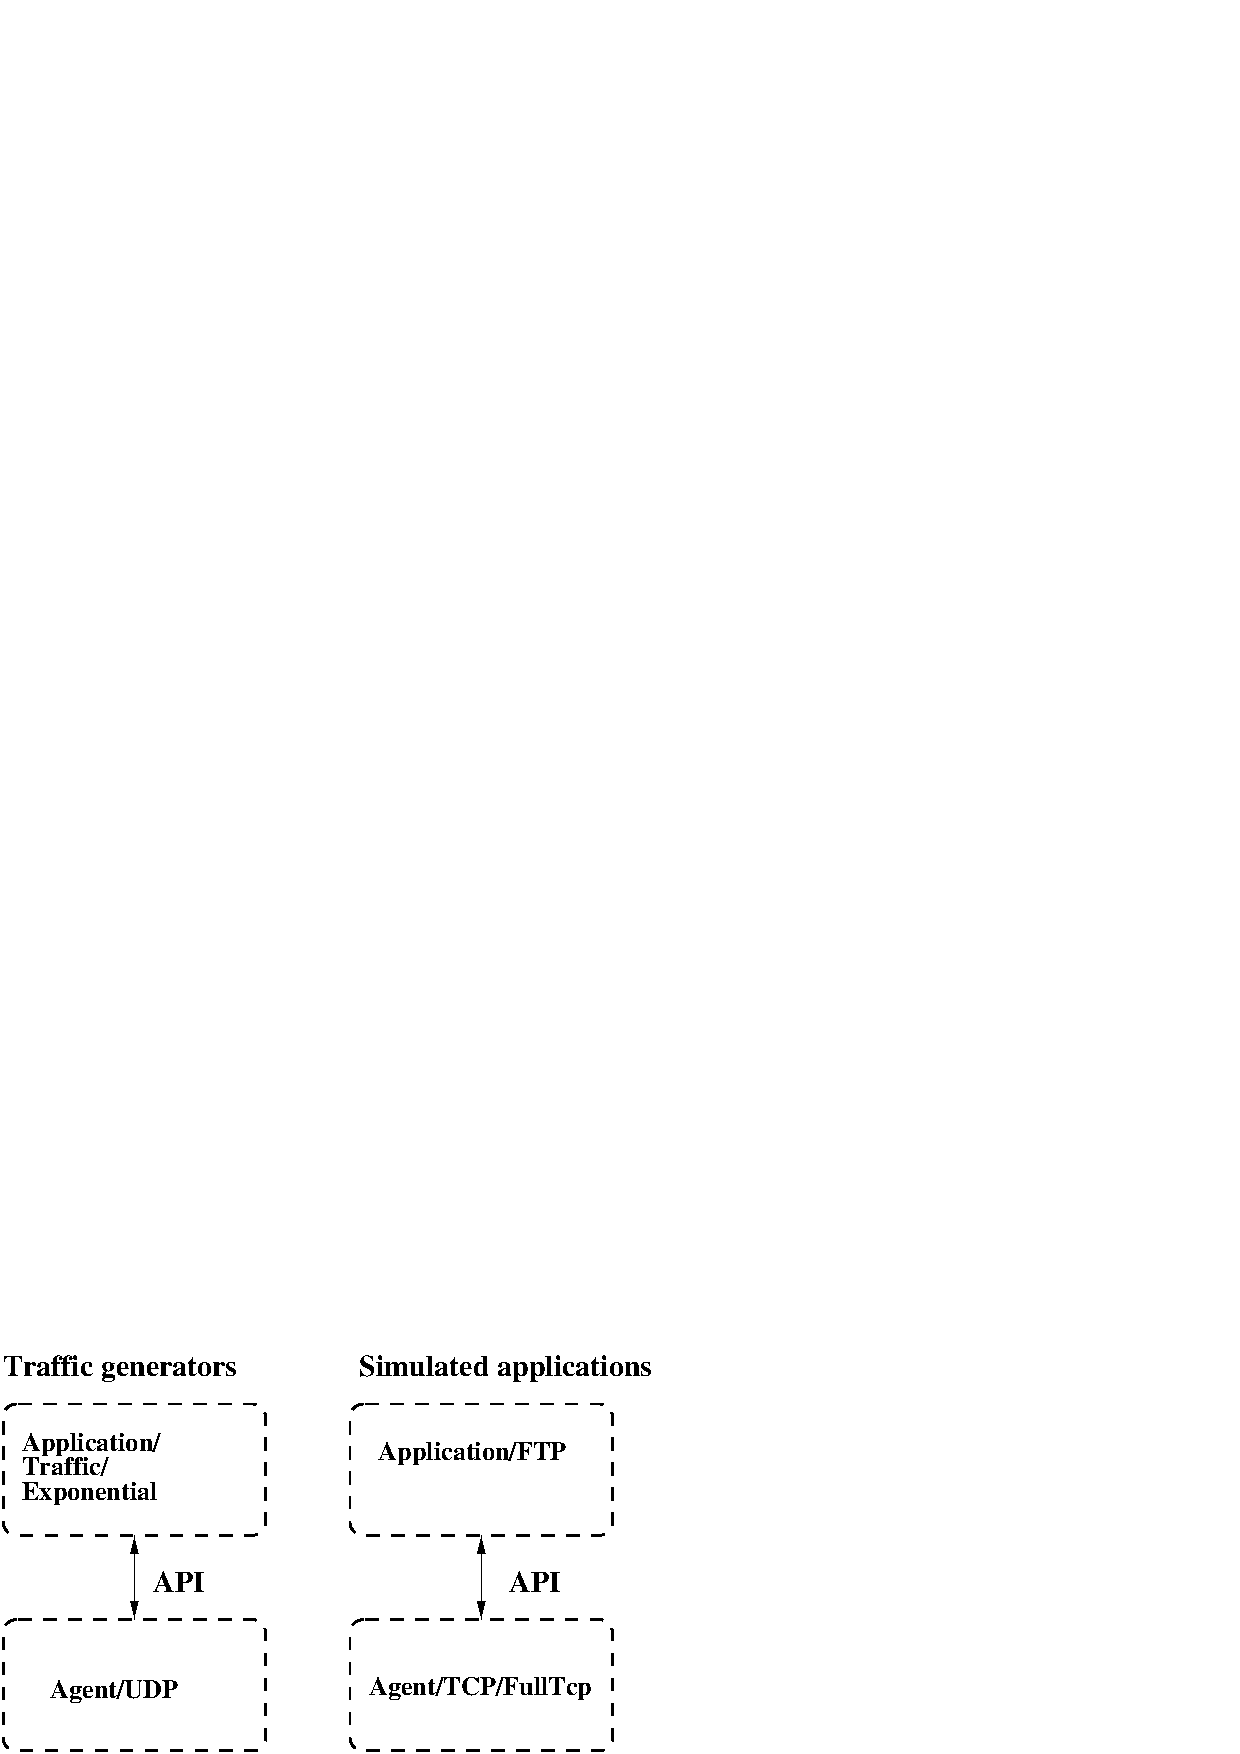
\includegraphics{application}}
  \caption{Example of Application Composition}
  \label{fig:application} 
\end{figure}

This chapter first describes the base \clsref{Application}{../ns-2/app.h}. 
Next, the transport API, through which applications request services from
underlying transport agents, is described.  Finally, the current 
implementations of traffic generators and sources are explained.  

%There are currently two methods of traffic generation in \ns.
%One method uses the abstract
%\clsref{TrafficGenerator}{../ns-2/trafgen.h}
%to generate inter-packet intervals and packet sizes.
%Currently, classes derived
%from TrafficGenerator are used in conjunction with the UDP\_Agent
%objects, which are responsible for actually allocating and
%transmitting the generated packets (Section~\ref{sec:trafgenclass}).
%The second method of traffic generation uses the Source class.
%Source objects generate traffic that is transported by TCPAgent objects
%(Section~\ref{sec:sourceobjects}).

\section{The class Application}
\label{sec:appclass}

Application is a C++ class defined as follows:
\begin{program}
        class Application : public TclObject \{
        public:
                Application();
                virtual void send(int nbytes);
                virtual void recv(int nbytes);
                virtual void resume();
        protected:
                int command(int argc, const char*const* argv);
                virtual void start();
                virtual void stop();
                Agent *agent_;
                int enableRecv_;                // call OTcl recv or not
                int enableResume_;              // call OTcl resume or not
        \};
\end{program}
Although objects of \code{class Application} are not meant to be instantiated,
we do not make it an abstract base class so that it is visible from OTcl level.
The class provides basic prototypes for application behavior 
(\code{send(), recv(), resume(), start(), stop()}), a pointer to the 
transport agent to which it is connected, and flags that indicate whether
a OTcl-level upcall should be made for \code{recv()} and 
\code{resume()} events.  

\section{The transport agent API}
In real-world systems, applications typically access network services through
an applications programming interface (API).  The most popular
of these APIs is known as ``sockets.''  In \ns, we mimic the behavior of the
sockets API through a set of well-defined API functions.  These functions 
are then mapped to the appropriate internal agent functions (e.g.,
a call to \code{send(numBytes)} causes TCP to increment its ``send buffer'' 
by a corresponding number of bytes).

This section describes how agents and applications are hooked together and
communicate with one another via the API.

\subsection{Attaching transport agents to nodes}
\label{sec:attachagentnode}
This step is typically done at OTcl level.  Agent management was also briefly
discussed in Section \ref{sec:node:node}.  

\begin{program}
        set src [new Agent/TCP/FullTcp]
        set sink [new Agent/TCP/FullTcp]
        $ns_ attach-agent $node_(s1) $src
        $ns_ attach-agent $node_(k1) $sink
        $ns_ connect $src $sink
\end{program}

The above code illustrates that in \ns, agents are first attached to a node
via \code{attach-agent}.  Next, the \code{connect} instproc sets each agent's
destination target to the other.  Note that, in \ns, \code{connect()} has
different semantics than in regular sockets.  In \ns, \code{connect()} simply
establishes the destination address for an agent, but does not set up the
connection.  As a result, the overlying application does not need to know
its peer's address.  For TCPs that exchange SYN segments, the first call to 
\code{send()} will trigger the SYN exchange. 

To detach an agent from a node, the instproc \code{detach-agent} can be 
used; this resets the target for the agent to a null agent.

\subsection{Attaching applications to agents}
\label{sec:attachappagent}

After applications are instantiated, they must be connected to a transport
agent.  The \code{attach-agent} method can be used to attach an application
to an agent, as follows:
\begin{program}
        set ftp1 [new Application/FTP]
        $ftp1 attach-agent $src
\end{program}

The following shortcut accomplishes the same result:
\begin{program}
        set ftp1 [$src attach-app FTP]
\end{program}

The attach-agent method, which is also used by attach-app, is implemented in 
C++.  It sets the \code{agent_}
pointer in \code{class Application} to point to the transport agent, and then
it calls \code{attachApp()} in \code{agent.cc} to set the \code{app_} pointer
to point back to the application.  By maintaining this binding only in C++,
OTcl-level instvars pointers are avoided and consistency between OTcl and C++ 
is guaranteed.  The OTcl-level command \code{[$ftp1 agent]} can be used by 
applications to obtain the handler for the transport agent.

\subsection{Using transport agents via system calls}
\label{sec:systemcalls}
Once transport agents have been configured and applications attached, 
applications can use transport 
services via the following system calls.  These calls can be invoked at either
OTcl or C++ level, thereby allowing applications to be coded in either C++ or
OTcl.  These functions have been implemented as virtual functions in the base
\code{class Agent}, and can be redefined as needed by derived Agents. 
\begin{itemize}
\item \code{send(int nbytes)}---Send nbytes of data to peer.  For TCP agents,
if \code{nbytes == -1}, this corresponds to an ``infinite'' send; i.e., the
TCP agent will act as if its send buffer is continually replenished by the
application.
\item \code{sendmsg(int nbytes, const char* flags = 0)}---Identical to 
\code{send(int nbytes)}, except that it passes an additional string 
\code{flags}.  Currently one flag value, ``MSG\_EOF,'' is defined; MSG\_EOF
specifies that this is the last batch of data that the application will 
submit, and serves as an implied close (so that TCP can send FIN with data).
\item \code{close()}---Requests the agent to close the connection (only 
applicable for TCP).
\item \code{listen()}---Requests the agent to listen for new connections
(only applicable for Full TCP).
\item \code{set_pkttype(int pkttype)}---This function sets the \code{type_} 
variable in the agent to \code{pkttype}.  Packet types are defined in 
\code{packet.h}.  This function is used to override the transport layer 
packet type for tracing purposes.  
\end{itemize}
Note that certain calls are not applicable for certain agents; e.g., a call
to \fcn[]{close} a UDP connection results in a no-op.  Additional calls
can be implemented in specialized agents, provided that they are made
\code{public} member functions. 

\subsection{Agent upcalls to applications}
\label{sec:upcalls}

Since presently in \ns~there is no actual data being passed between 
applications, agents can instead announce to applications the occurrence of 
certain events at the transport layer through ``upcalls.''  For example,
applications can be notified of the arrival of a number of bytes of data;
this information may aid the application in modelling real-world application
behavior more closely.  Two basic ``upcalls'' have been implemented in 
base \code{class Application} and in the transport agents:
\begin{itemize} 
\item \code{recv(int nbytes)}---Announces that \code{nbytes} of data have been
received by the agent.  For UDP agents, this signifies the arrival of
a single packet.  For TCP agents, this signifies the ``delivery'' of an 
amount of in-sequence data, which may be larger than that contained in a 
single packet (due to the possibility of network reordering).
\item \code{resume()}---This indicates to the application that the transport
agent has sent out all of the data submitted to it up to that point in time.  
For TCP, it does not indicate whether the data has been ACKed yet, only that
it has been sent out for the first time. 
\end{itemize}
The default behavior is as follows: 
Depending on whether the application has been implemented in C++ or OTcl, these
C++ functions 
call a similarly named (\code{recv, resume}) function in the application,
if such methods have been defined.   

Although strictly not a callback to applications, certain Agents have
implemented a callback from C++ to OTcl-level that has been used by 
applications such as HTTP simulators.  This callback method, \code{done\{\}},
is used in TCP agents.  In TCP, \code{done\{\}} is called when a TCP sender 
has received ACKs for all of its data and is now closed; it therefore can
be used to simulate a blocked TCP connection.  The \code{done\{\}}
method was primarily used before this API was completed, but may still be
useful for applications that do not want to use \code{resume()}.

To use \code{done\{\}} for FullTcp, for example, you can try:
\begin{program}
        set myagent [new Agent/TCP/FullTcp]
        $myagent proc done { } {
            ... code you want ...
        }
\end{program}
If you want all the FullTCP's to have the same code you could also do:
\begin{program}
        Agent/TCP/FullTcp instproc done {} {
            ... code you want ...
        }
\end{program}
By default, \code{done\{\}} does nothing.

\subsection{An example}
\label{sec:syscallsexample}
Here is an example of how the API is used to implement a simple application
(FTP) on top of a FullTCP connection. 

\begin{program}
        set src [new Agent/TCP/FullTcp]
        set sink [new Agent/TCP/FullTcp]
        $ns_ attach-agent $node_(s1) $src
        $ns_ attach-agent $node_(k1) $sink
        $ns_ connect $src $sink

        # set up TCP-level connections
        $sink listen; 
        $src set window_ 100

        set ftp1 [new Application/FTP]
        $ftp1 attach-agent $src

        $ns_ at 0.0 "$ftp1 start"
\end{program}

In the configuration script, the first five lines of code allocates two new
FullTcp agents, attaches them to the correct nodes, and "connects" them
together (assigns the correct destination addresses to each agent).  The
next two lines configure the TCP agents further, placing one of them in
LISTEN mode.  Next, \code{ftp1} is defined as a new FTP Application, and 
the \code{attach-agent} method is called in C++ (\code{app.cc}).     

The ftp1 application is started at time 0:
\begin{program}
        Application/FTP instproc start \{\} \{
      	        [$self agent] send -1;   # Send indefinitely
        \}
\end{program}
Alternatively, the FTP application could have been implemented in C++ as
follows:
\begin{program}
        void FTP::start()
        \{
                agent_->send(-1);    // Send indefinitely
        \}
\end{program}  
Since the FTP application does not make use of callbacks, these functions
are null in C++ and no OTcl callbacks are made. 

\section{The class TrafficGenerator}
\label{sec:trafgenclass}

TrafficGenerator is an abstract C++ class defined as follows:
\begin{program}
        class TrafficGenerator : public Application \{
        public:
                TrafficGenerator();
                virtual double next_interval(int &) = 0;
                virtual void init() \{\}
                virtual double interval() \{ return 0; \}
                virtual int on() \{ return 0; \}
                virtual void timeout();
                virtual void recv() \{\}
                virtual void resume() \{\}
        protected:
                virtual void start();
                virtual void stop();
                double nextPkttime_;
                int size_;
                int running_;
                TrafficTimer timer_;
        \};
\end{program}
The pure virtual function \fcn[]{next\_interval} returns the time until the
next packet is created and also sets the size in bytes of the next
packet.  The function \fcn[]{start} calls \fcn{init} and starts the 
timer.  The function \fcn[]{timeout} sends a packet and reschedules the
next timeout.  The function \fcn[]{stop} cancels any pending transmissions.
Callbacks are typically not used for traffic generators, so these 
functions (\code{recv, resume}) are null.

Currently, there are four C++ classes derived from the
class TrafficGenerator:
\begin{enumerate}
\item \code{EXPOO_Traffic}---generates traffic according to an
  Exponential On/Off distribution.
  Packets are sent at a fixed rate during on periods, and
  no packets are sent during off periods.
  Both on and off periods are taken from an exponential distribution.
  Packets are constant size.
\item \code{POO_Traffic}---generates traffic
  according to a Pareto On/Off distribution.
  This is identical to the Exponential On/Off distribution,
  except the on and off periods are taken from a pareto distribution.
  These sources can be used to generate aggregate traffic
  that exhibits long range dependency.
\item \code{CBR_Traffic}---generates traffic according to a deterministic rate.
  Packets are constant size.  Optionally, some randomizing dither can be
  enabled on the interpacket departure intervals. 
\item \code{TrafficTrace}---generates traffic according to a trace file.
  Each record in the trace file consists of 2 32-bit fields
   in network (big-endian) byte order.
  The first contains the time in microseconds
  until the next packet is generated.
  The second contains the length in bytes of the next packet.
\end{enumerate}
These classes can be created from OTcl.  The OTcl classes names and
associated parameters are given below:

\paragraph{Exponential On/Off}
An Exponential On/Off object is embodied in the OTcl class
Application/Traffic/Exponential.  The member variables that parameterize this
object are:
\begin{alist}
\code{packetSize\_} & the constant size of the packets generated\\
\code{burst\_time\_} & the average ``on'' time for the generator\\
\code{idle\_time\_} & the average ``off'' time for the generator\\
\code{rate\_} & the sending rate during ``on'' times\\
\end{alist}
Hence a new Exponential On/Off traffic generator can be created and 
parameterized as follows:
\begin{program}
        set e [new Application/Traffic/Exponential]
        $e set packetSize_ 210
        $e set burst_time_ 500ms
        $e set idle_time_ 500ms
        $e set rate_ 100k
\end{program}

{\bf NOTE:} The Exponential On/Off generator can be configured to behave
as a {\bf Poisson process} by setting the variable \code{burst_time_} to \code{0}
and the variable \code{rate_} to a very large value.  The C++ code
guarantees that even if the burst time is zero, at least one packet is
sent.  Additionally, the next interarrival time is the sum of the
assumed packet transmission time (governed by the variable \code{rate_}) and 
the random variate corresponding to \code{idle_time_}.  
Therefore, to make the first term in the sum very small, make the burst
rate very large so that the transmission time is negligible compared to
the typical idle times.

\paragraph{Pareto On/Off}
A Pareto On/Off object is embodied in the OTcl class Application/Traffic/Pareto.
The member variables that parameterize this object are:
\begin{alist}
\code{packetSize\_} & the constant size of the packets generated\\
\code{burst\_time\_} & the average "on" time for the generator\\
\code{idle\_time\_} & the average "off" time for the generator\\
\code{rate\_} & the sending rate during "on" times\\
\code{shape\_} & the "shape" parameter used by the pareto distribution\\
\end{alist}
A new Pareto On/Off traffic generator can be created as follows:
\begin{program}
        set p [new Application/Traffic/Pareto]
        $p set packetSize_ 210
        $p set burst_time_ 500ms
        $p set idle_time_ 500ms
        $p set rate_ 200k
        $p set shape_ 1.5
\end{program}

\paragraph{CBR}
A CBR  object is embodied in the OTcl class
Application/Traffic/CBR.  The member variables that parameterize this
object are:  
\begin{alist}
\code{rate\_} & the sending rate \\
\code{interval\_} & (Optional) interval between packets \\
\code{packetSize\_} & the constant size of the packets generated\\
\code{random\_} & flag indicating whether or not to introduce random ``noise'' 
in the scheduled departure times (default is off)\\
\code{maxpkts\_} & the maximum number of packets to send (default is (\(2^28\))\\
\end{alist}
Hence a new CBR traffic generator can be created and parameterized
as follows:
\begin{program}
        set e [new Application/Traffic/CBR]
        $e set packetSize_ 48
        $e set rate_ 64Kb
        $e set random_ 1
\end{program}

The setting of a CBR object's \code{rate_} and \code{interval_} are mutually
exclusive (the interval between packets is maintained as an interval 
variable in C++,
and some example \ns~scripts specify an interval rather than a rate).  In
a simulation, either a rate or an interval (but not both) should be 
specified for a CBR object.  

\paragraph{Traffic Trace}
A Traffic Trace object is instantiated by the OTcl class 
Application/Traffic/Trace.
The associated class Tracefile is used to enable multiple 
Traffic/Trace objects to be associated with a single trace file.
The Traffic/Trace class uses the method attach-tracefile to associate
a Traffic/Trace object with a particular Tracefile object.
The method filename of the Tracefile class associates a trace file
with the Tracefile object.
The following example shows how to create two Application/Traffic/Trace objects,
each associated with the same trace file
(called "example-trace" in this example).
To avoid synchronization of the traffic generated,
random starting places within the trace file are chosen for
each Traffic/Trace object.
\begin{program}
        set tfile [new Tracefile]
        $tfile filename example-trace

        set t1 [new Application/Traffic/Trace]
        $t1 attach-tracefile $tfile
        set t2 [new Application/Traffic/Trace]
        $t2 attach-tracefile $tfile
\end{program}

\subsection{An example}

The following code illustrates the basic steps to configure an Exponential
traffic source over a UDP agent, for traffic flowing from node \code{s1} to 
node \code{k1}:

\begin{program}
        set src [new Agent/UDP]
        set sink [new Agent/UDP]
        $ns_ attach-agent $node_(s1) $src
        $ns_ attach-agent $node_(k1) $sink
        $ns_ connect $src $sink
	
        set e [new Application/Traffic/Exponential]
        $e attach-agent $src
        $e set packetSize_ 210
        $e set burst_time_ 500ms
        $e set idle_time_ 500ms
        $e set rate_ 100k

        $ns_ at 0.0 "$e start"
\end{program}

\section{Simulated applications:  Telnet and FTP}
\label{sec:simapps}
 
There are currently two ``simulate application'' classes derived from 
Application:
Application/FTP and Application/Telnet.  These classes work by advancing the
count of packets available to be sent by a TCP transport agent.
The actual transmission of available packets is still controlled by TCP's flow 
and congestion control algorithm.
 
\paragraph{Application/FTP} 
Application/FTP, implemented in OTcl, simulates bulk data transfer.  
The following are methods of the Application/FTP class:
\begin{alist}
\code{attach-agent} & attaches an Application/FTP object to an agent.\\ 
\code{start} & start the Application/FTP by calling the TCP agent's 
\code{send(-1)} function, which causes TCP to behave as if the application 
were continuously sending new data.\\
\code{stop} & stop sending.\\ 
\code{produce n} &  set the counter of packets to be sent to $n$.\\ 
\code{producemore n} &  increase the counter of packets to be sent by $n$. \\
\code{send n} & similar to \code{producemore}, but sends $n$ bytes instead of
packets.  
\end{alist} 

\paragraph{Application/Telnet} 
Application/Telnet objects generate packets in one of two ways.
If the member variable \code{interval_} is non-zero,
then inter-packet times are chosen
from an exponential distribution with average equal to \code{interval_}.
If \code{interval_} is zero, then inter-arrival times are chosen
according to the tcplib distribution (see tcplib-telnet.cc).
The start method starts the packet generation process.

\section{Applications objects} 
\label{sec:appobjects} 
An application object may be of two types, a traffic generator or a
simulated application. Traffic generator objects generate traffic and can
be of four types, namely, exponential, pareto, CBR and traffic trace. 
\begin{description} 
\item[Application/Traffic/Exponential objects]
Exponential traffic objects generate On/Off traffic. During "on" periods,
packets are generated at a constant burst rate. During "off" periods, no
traffic is generated. Burst times and idle times are taken from
exponential distributions. Configuration parameters are:  
\begin{description} 
\item[PacketSize\_] constant size of packets generated.
\item[burst\_time\_] average on time for generator. 
\item[idle\_time\_] average off time for generator.  
\item[rate\_] sending rate during on time.  
\end{description}

\item[Application/Traffic/Pareto] 
Application/Traffic/Pareto objects generate On/Off traffic with burst
times and idle times taken from pareto distributions. Configuration
parameters are:
\begin{description}
\item[PacketSize\_] constant size of packets generated.
\item[burst\_time\_] average on time for generator.
\item[idle\_time\_] average off time for generator.
\item[rate\_] sending rate during on time.
\item[shape\_] the shape parameter used by pareto distribution.
\end{description}

\item[Application/Traffic/CBR]
CBR objects generate packets at a constant bit rate. 

\code{$cbr start}\\
Causes the source to start generating packets. 

\code{$cbr stop}\\
Causes the source to stop generating packets. 

Configuration parameters are:
\begin{description}
\item[PacketSize\_] constant size of packets generated. 
\item[rate\_] sending rate.
\item[interval\_] (optional) interval between packets.
\item[random\_] whether or not to introduce random noise in the scheduled
departure times. defualt is off.
\item[maxpkts\_] maximum number of packets to send.
\end{description}

\item[Application/Traffic/Trace]
Application/Traffic/Trace objects are used to generate traffic from a
trace file. 
\code{$trace attach-tracefile tfile}\\
Attach the Tracefile object tfile to this trace. The Tracefile object
specifies the trace file from which the traffic data is to be read.
Multiple Application/Traffic/Trace objects can be attached
to the same Tracefile object. A random starting place within the Tracefile
is chosen for each Application/Traffic/Trace object. \\

There are no configuration parameters for this object. 
\end{description}

A simulated application object can be of two types, Telnet and FTP.
\begin{description}
\item[Application/Telnet]
TELNET objects produce individual packets with inter-arrival times as
follows. If interval\_ is non-zero, then inter-arrival times are chosen
from an exponential distribution with average interval\_. If interval\_ is
zero, then inter-arrival times are chosen using the "tcplib" telnet
distribution. 

\code{$telnet start}\\
Causes the Application/Telnet object to start producing packets. 

\code{$telnet stop}\\
Causes the Application/Telnet object to stop producing packets. 

\code{$telnet attach <agent>}\\
Attaches a Telnet object to agent. 

Configuration Parameters are:
\begin{description}

\item[interval\_]
The average inter-arrival time in seconds for packets generated by the
Telnet object. 
\end{description}


\item[Application FTP]
FTP objects produce bulk data for a TCP object to send. 

\code{$ftp start}\\
Causes the source to produce maxpkts\_ packets. 

\code{$ftp produce <n>}\\
Causes the FTP object to produce n packets instantaneously. 

\code{$ftp stop}\\
Causes the attached TCP object to stop sending data. 

\code{$ftp attach agent}\\
Attaches a Application/FTP object to agent. 

\code{$ftp producemore <count>}\\
Causes the Application/FTP object to produce count more packets. 

Configuration Parameters are:
\begin{description}
\item[maxpkts] The maximum number of packets generated by the source. 
\end{description}
\end{description}

\textsc{Tracefile objects}
Tracefile objects are used to specify the trace file that is to be used
for generating traffic (see Application/Traffic/Trace objects
described earlier in this section). \code{$tracefile} is an instance of
the Tracefile Object. 
\code{$tracefile filename <trace-input>}\\
Set the filename from which the traffic trace data is to be read to
trace-input. 

There are no configuration parameters for this object. A trace file
consists of any number of fixed length records. Each record consists of 2
32 bit fields. The first indicates the interval until the next packet is
generated in microseconds. The second indicates the length of the next
packet in bytes. 



\section{Commands at a glance}
\label{sec:appscommand}

Following are some transport agent and application related commands
commonly used in simulation scripts:
\begin{flushleft}
\begin{program}
set tcp1 [new Agent/TCP]
$ns_ attach-agent $node_(src) $tcp1
set sink1 [new Agent/TCPSink]
$ns_ attach-agent $node_(snk) $sink1
$ns_ connect $tcp1 $sink1
\end{program}
This creates a source tcp agent and a destination sink agent. Both the transport
agents are attached to their resoective nodes. Finally an end-to-end connection
is setup between the src and sink.


\begin{program}
set ftp1 [new Application/FTP]
$ftp1 attach-agent $agent
\end{program}
or
\code{set ftp1 [$agent attach-app FTP]}
Both the above commands achieve the same. An application (ftp in this example)
is created and attached to the source agent. An application can be of two
types, a traffic generator or a simulated application.
Types of Traffic generators currently present are: 
Application/Traffic/Exponential, Application/Traffic/Pareto,
Application/Traffic/CBR, and Application/Traffic/Trace. See section \ref{sec:trafgenclass}
for details.
Types of simulated applications currently implemented are:
Application/FTP and Application/Telnet. See  section \ref{sec:simapps} for
details.

\end{flushleft}

\endinput
